

\begin{figure}[h!]
	\centering
 	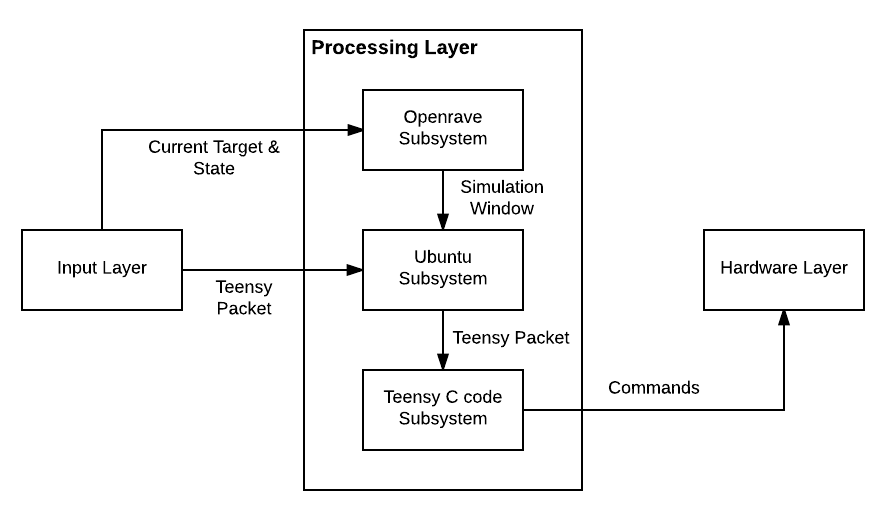
\includegraphics[width=0.60\textwidth]{images/processing}
 \caption{Processing Layer subsystem diagram}
\end{figure}

\subsection{OpenRave Subsystem}
The OpenRave Subsystem will simulate the movement of the robot arm and calculate the kinematics to find the optimal path to send to the arm.

\subsubsection{Assumptions}
The OpenRave subsystem will be able to simulate the arm accurately and be able to make accurate calculations

\subsubsection{Responsibilities}
This subsystem is responsible for using the simulation as well as calculate the kinematics needed to find the most accurate path for the robot arm to take, and is also responsible for communicating this data to the system.

\subsubsection{OpenRave Interfaces}

\begin {table}[H]
\caption {Subsystem interfaces} 
\begin{center}
    \begin{tabular}{ | p{1cm} | p{6cm} | p{3cm} | p{3cm} |}
    \hline
    ID & Description & Inputs & Outputs \\ \hline
    \#1 & Data in the form of a packet & \pbox{3cm}{Current target and state} & \pbox{3cm}{None}  \\ \hline
    \#2 & Simulation Window data & \pbox{3cm}{N/A} & \pbox{3cm}{Simulation window}  \\ \hline
    \end{tabular}
\end{center}
\end{table}

\subsection{Ubuntu Subsystem}
The Ubuntu Subsystem is what hosts the GUI and OpenRave simulation and sends data to the Teensy board.

\subsubsection{Assumptions}
The Ubuntu subsystem will be able to adequately host the application and be able to communicate with the Teensy board

\subsubsection{Responsibilities}
This subsystem is responsible for hosting the application and simulation while communicating with the Teensy board through a USB connection.

\subsubsection{Subsystem Interfaces}

\begin {table}[H]
\caption {Ubuntu interfaces} 
\begin{center}
    \begin{tabular}{ | p{1cm} | p{6cm} | p{3cm} | p{3cm} |}
    \hline
    ID & Description & Inputs & Outputs \\ \hline
    \#1 & Data in the form of a packet & \pbox{3cm}{Teensy Packet (from the GUI)} & \pbox{3cm}{Teensy Packet (to the Teensy)}  \\ \hline
    \#2 & Simulation Window data & \pbox{3cm}{N/A} & \pbox{3cm}{Simulation window display}  \\ \hline
    \end{tabular}
\end{center}
\end{table}

\subsection{Teensy C-Code Subsystem}
The Teensy C Code subsystem has the code to send commands to the hardware.

\subsubsection{Assumptions}
The Teensy C Code subsystem will be coded to send commands to operate the hardware accurately.

\subsubsection{Responsibilities}
This subsystem is responsible for receiving the packet data and using it to communicate with and send commands to the hardware subsystems to operate them. 

\subsubsection{Subsystem Interfaces}

\begin {table}[H]
\caption {Teensy interfaces} 
\begin{center}
    \begin{tabular}{ | p{1cm} | p{6cm} | p{3cm} | p{3cm} |}
    \hline
    ID & Description & Inputs & Outputs \\ \hline
    \#1 & Data in the form of a packet & \pbox{3cm}{Teensy packet data} & \pbox{3cm}{None}  \\ \hline
    \#2 & Command data & \pbox{3cm}{N/A} & \pbox{3cm}{Commands}  \\ \hline
    \end{tabular}
\end{center}
\end{table}